\documentclass[draft=True]{thesis}
\documentclass[a4paper,10pt,draft]{thesis}
\usepackage{physics,amsmath, amsfonts, siunitx, amssymb, graphicx, slashed,subcaption}
\usepackage[utf8]{inputenc}
\usepackage[margin=1in]{geometry}
\usepackage[hidelinks]{hyperref}
\usepackage{xr-hyper}
\newcommand{\n}[1]{\nu_{#1}}
\newcommand{\na}{\nu_\alpha}
\newcommand{\nb}{\nu_\beta}
\newcommand{\ana}{\bar{\nu}_\alpha}
\newcommand{\an}[1]{\bar{\nu}_{\text{#1}}}
\newcommand{\anb}{\bar{\nu}_\beta}
\renewcommand{\a}{\alpha}
\renewcommand{\b}{\beta}
\newcommand{\ab}{\alpha\beta}


\renewcommand{\ne}{\nu_e}
\newcommand{\nm}{\nu_\mu}
\newcommand{\nt}{\nu_\tau}
\newcommand{\ns}{\nu_s}

\newcommand{\ane}{\bar{\nu}_e}
\newcommand{\anm}{\bar{\nu}_\mu}
\newcommand{\ant}{\bar{\nu}_\tau}
\newcommand{\ans}{\bar{\nu}_s}

\newcommand{\nee}{\nu_e \to \nu_e}
\newcommand{\nem}{\nu_e \to \nu_\mu}
\newcommand{\net}{\nu_e \to \nu_\tau}
\newcommand{\nes}{\nu_e \to \nu_s}

\newcommand{\nme}{\nu_\mu \to \nu_e}
\newcommand{\nmm}{\nu_\mu \to \nu_\mu}
\newcommand{\nmt}{\nu_\mu \to \nu_\tau}
\newcommand{\nms}{\nu_\mu \to \nu_s}



\newcommand{\Pee}{P_{e  e}}
\newcommand{\Pem}{P_{e  \mu}}
\newcommand{\Pet}{P_{e  \tau}}
\newcommand{\Pes}{P_{e  s}}

\newcommand{\Pme}{P_{\mu  e}}
\newcommand{\Pmm}{P_{\mu\mu}}
\newcommand{\Pmt}{P_{\mu  \tau}}
\newcommand{\Pms}{P_{\mu  s}}


\newcommand{\Pte}{P_{P_{\tau e}}}
\newcommand{\Ptm}{P_{\tau  \mu}}
\newcommand{\Ptt}{P_{\tau  \tau}}
\newcommand{\Pts}{P_{\mu  s}}

\newcommand{\Paeae}{P_{\bar{e}  \bar{e}}}
\newcommand{\Paeam}{P_{\bar{e}  \bar{\mu}}}
\newcommand{\Paeat}{P_{\bar{e}  \bar{\tau}}}
\newcommand{\Paeas}{P_{\bar{e}  \bar{s}}}

\newcommand{\Pamae}{P_{\bar{\mu}  \bar{e}}}
\newcommand{\Pamam}{P_{\bar{\mu}  \bar{\mu}}}
\newcommand{\Pamat}{P_{\bar{\mu}  \bar{\tau}}}
\newcommand{\Pamas}{P_{\bar{\mu}  \bar{s}}}


\newcommand{\Patae}{P_{\bar{\tau}  \bar{e}}}
\newcommand{\Patam}{P_{\bar{\tau}  \bar{\mu}}}
\newcommand{\Patat}{P_{\bar{\tau}  \bar{\tau}}}
\newcommand{\Patas}{P_{\bar{\mu}  \bar{s}}}

\renewcommand{\th}[1][]{%
  \theta\ifx\\#1\\\else_\text{#1}\fi
}
\newcommand{\thm}[1][]{%
  \theta^\text{M}\ifx\\#1\\\else_\text{#1}\fi
}
\renewcommand{\t}[1]{\text{{#1}}}
\newcommand{\avg}[1]{\left\langle {#1} \right \rangle}
\newcommand*{\dm}[1][]{%
  \Delta m^2\ifx\\#1\\\else_\text{#1}\fi
}
\newcommand{\zreco}{\cos{(\theta_z^{reco})}}
\newcommand{\ztrue}{\cos{(\theta_z^{true})}}
\newcommand{\z}{\cos{(\theta_z)}}
\newcommand{\Ereco}{E^{reco}}
\newcommand{\Etrue}{E^{true}}
\newcommand{\Aeff}{A^\text{eff}}
\newcommand{\emm}{\epsilon_{\mu\mu}}
\newcommand{\emt}{\epsilon_{\mu\tau}}
\newcommand{\eet}{\epsilon_{e\tau}}
\newcommand{\eem}{\epsilon_{e\mu}}
\newcommand{\ett}{\epsilon_{\tau\tau}}
\newcommand{\ep}{\epsilon^\prime}

\usepackage{physics,amsmath, amsfonts, siunitx, amssymb, graphicx}
\usepackage[utf8]{inputenc}
\usepackage{xr-hyper}


\begin{document}
\section{How NSIs alter the matter potential}
Up until now, we have only considered neutrino interactions with electrons, protons, and neutrons. Now we extend this to include we can extend this to include 
the up and down quarks which are present in the Earth as the fundamental components of neutrons and protons. 
Consider interactions beyond the Standard Model through the following Lagrangians,
\begin{align*}
    \mathcal{L}_{\mathrm{CC}} &= -2 \sqrt{2} G_{F} \epsilon_{\alpha \beta}^{f f^{\prime} X}\left(\bar{\nu}_{\alpha} \gamma^{\mu} P_{L} \ell_{\beta}\right)\left(\bar{f}^{\prime} \gamma_{\mu} P_{X} f\right) \\
    \mathcal{L}_{\mathrm{NC}} &= -2 \sqrt{2} G_{F} \epsilon_{\alpha \beta}^{f X}\left(\bar{\nu}_{\alpha} \gamma^{\mu} P_{L} \nu_{\beta}\right)\left(\bar{f} \gamma_{\mu} P_{X} f\right)\,,
\end{align*}
where CC denotes the charged current interaction with the matter field $f\neq f^\prime \in \{u,d\}$, and NC denotes the neutral current interaction with 
$f \in \{e,u,d\}$. 

We have no independent sensitivity for the neither chirality nor flavor type of $\epsilon^X$, so we sum over these and study the effective matter NSI parameter
 $\epsilon_{\ab}$:
\begin{align}
    \epsilon_{\ab} = \sum_{X \in \{L,R\}} \sum_{f \in \{e,u,d\}} \frac{N_f}{N_e} \epsilon^{fX}_{\ab}\,.
\end{align}
Our matter study will be wholly confined to the interior of the Earth, where we assume electrical neutrality and equal distribution of neutrons and protons, 
we get $N_u/N_e \simeq U_d/N_e \simeq 3$. Also we assume the components $\epsilon_{\a\b}$ to be real. Thus,
\begin{align}
    \epsilon_{\ab} =  \sum_X [\epsilon_{\ab}^{eX} + 3(\epsilon_{\ab}^{uX} + \epsilon_{\ab}^{dX})]
\end{align}
Now, $\epsilon_{\ab}$ enters the Hamiltonian as entries of a potential-like matrix. In Eq.~\ref{eq:NSIH}, $A_{CC}\text{diag}(1,0,0)$ is our 
familiar matter potential from the Standard Model. There is also our new term, $A_{CC} \epsilon$, which contains the components $\epsilon_{\a\b}$:
\begin{align}\label{eq:NSIH}
    H &= \frac{1}{2E} \left[UM^2U^\dagger + A_{CC}\text{diag}(1,0,0) + A_{CC} \epsilon \right] \nonumber \\
      &= \frac{1}{2E} \left[UM^2U^\dagger + A_{CC}
      \begin{pmatrix}
          1 + \epsilon_{ee} & \epsilon_{e\mu} & \epsilon_{e\tau}  \\
          \epsilon_{\mu e} & \epsilon_{\mu\mu} & \epsilon_{\mu\tau}  \\
          \epsilon_{\tau e} & \epsilon_{\tau\mu} & \epsilon_{\tau\tau}
      \end{pmatrix} \right]\,.
\end{align} 
In the limit $\epsilon_{\ab} \to 0$, we recover the standard interaction Hamiltonian from Eq.~\ref{eq:H_3gen}.
We can draw several conclusions from this form of the Hamiltonian. Any nonzero off-diagonal element $\epsilon_{\ab}, \a \neq \b$ will make the NSI violate 
lepton flavor, just as the off-diagonal elements of $U$ does in the SM. Moreover, since the SM potential has the same order in $A_{CC}$ as the NSIs, 
any $\epsilon_{\ab} \sim 1$ will make the new matter effect be the same order as the SM effect.
Regarding the source of these new parameters, $\epsilon_{\ab}$ have the scale
\begin{align}
    \epsilon_{\ab} \propto \frac{m_W^2}{m_{\epsilon}^2} \sim \frac{10^{-2}}{m_\epsilon^2}\,
\end{align} 
in TeV, so the new interactions generated at a mass scale of $m_\epsilon = \SI{1}{TeV}$ will produce NSI parameters in the order of $10^{-2}$, 
two magnitudes below the SM matter effect. Thus, if we assume the new interactions to arise from a higher-energy theory at or above TeV scale, 
we then predict that the NSI parameters contribute at most $10^{-2}$ to the SM matter effect, decreasing quadratically.

We have two more modifications to the matrix $\epsilon$. First, all terms of the Hamiltonian must of course be Hermitian, thus
\begin{align}
    \begin{pmatrix}
        \epsilon_{ee} & \epsilon_{e\mu} & \epsilon_{e\tau}  \\
        \epsilon_{\mu e} & \epsilon_{\mu\mu} & \epsilon_{\mu\tau}  \\
        \epsilon_{\tau e} & \epsilon_{\tau\mu} & \epsilon_{\tau\tau}
    \end{pmatrix} =
    \begin{pmatrix}
        \epsilon_{ee} & \epsilon_{e\mu} & \epsilon_{e\tau}  \\
        \epsilon_{e \mu} & \epsilon_{\mu\mu} & \epsilon_{\mu\tau}  \\
        \epsilon_{e\tau} & \epsilon_{\mu\tau} & \epsilon_{\tau\tau}
    \end{pmatrix}\,.
\end{align}
Now we have reduced the possible number of NSI parameters from 9 down to 6. Moreover, it is common to subtract $\emm$ from the diagonal, which
we are free to do since any multiple added or subtracted from diagonal does not affect the eigenvectors of the Hamiltonian and thus not the
probabilities. So just as we subtracted away $V_{NC}$ back in Eq.~\ref{eq:components}, we can subtract $\emm$ and rotate it away.
Our NSI potential matrix now takes the form 
\begin{align}
    \begin{pmatrix}
        \epsilon_{ee} & \epsilon_{e\mu} & \epsilon_{e\tau}  \\
        \epsilon_{e \mu} & \epsilon_{\mu\mu} & \epsilon_{\mu\tau}  \\
        \epsilon_{e\tau} & \epsilon_{\mu\tau} & \epsilon_{\tau\tau}
    \end{pmatrix} 
    - \epsilon_{\mu\mu}
    \begin{pmatrix}
        1 & 0 & 0 \\
        0 & 1 & 0 \\
        0 & 0 & 1 
    \end{pmatrix}
     &= \begin{pmatrix}
        \epsilon_{ee}- \epsilon_{\mu\mu} & \epsilon_{e\mu} & \epsilon_{e\tau}  \\
        \epsilon_{e \mu} & 0 & \epsilon_{\mu\tau}  \\
        \epsilon_{e\tau} & \epsilon_{\mu\tau} & \epsilon_{\tau\tau} - \epsilon_{\mu\mu}
    \end{pmatrix} \nonumber \\
    &= \begin{pmatrix}
        \epsilon_{ee}- \epsilon_{\mu\mu} & \epsilon_{e\mu} & \epsilon_{e\tau}  \\
        \epsilon_{e \mu} & 0 & \epsilon_{\mu\tau}  \\
        \epsilon_{e\tau} & \epsilon_{\mu\tau} & \ep
    \end{pmatrix}\,,
\end{align}
where $\ep = \ett - \emm$.

\section{Non-standard interactions in IceCube}
In our analysis of IceCube, we are constrained to muon track events. Thus, we are not able to test any theory which does not modify $P_{\a \mu}$ directly or 
indirectly. Since all standard matter potentials are diagonal, the elements $\epsilon_{\a\a}$ will directly adjust the matter potential felt 
by flavor $\a$. The off-diagonal terms have a more interesting implication. %TODO: fill
In Fig.~\ref{fig:IC_NSI_probs}, we plot $\Pmm$ and $\Pamam$ for 3 cases of $\ep$ and $\emt$ each. As is clear from the 
left panels, the value of $\ett$ does not affect neither $\Pmm$ nor $\Pamam$, as we expected. Hence, we will not be able
to say anything about $\ett$ in our study. The right panels show an interesting relationship between the sign of the NSI parameter 
and the neutrino type. $\Pmm$ with positive $\ett$ is the same as $\Pamam$ with negative $\ett$. Looking at the form of the matter potential, 
this is something that we should expect. In the standard interaction framework, we distinguish between neutrinos and antineutrinos by flipping the sign 
of the CC potential. Since the NSI potential has the same form, any sign flipping of the NSI potential will have the same effect as 
having an antineutrino.

\begin{figure}\label{fig:IC_NSI_probs}
    \begin{center}
    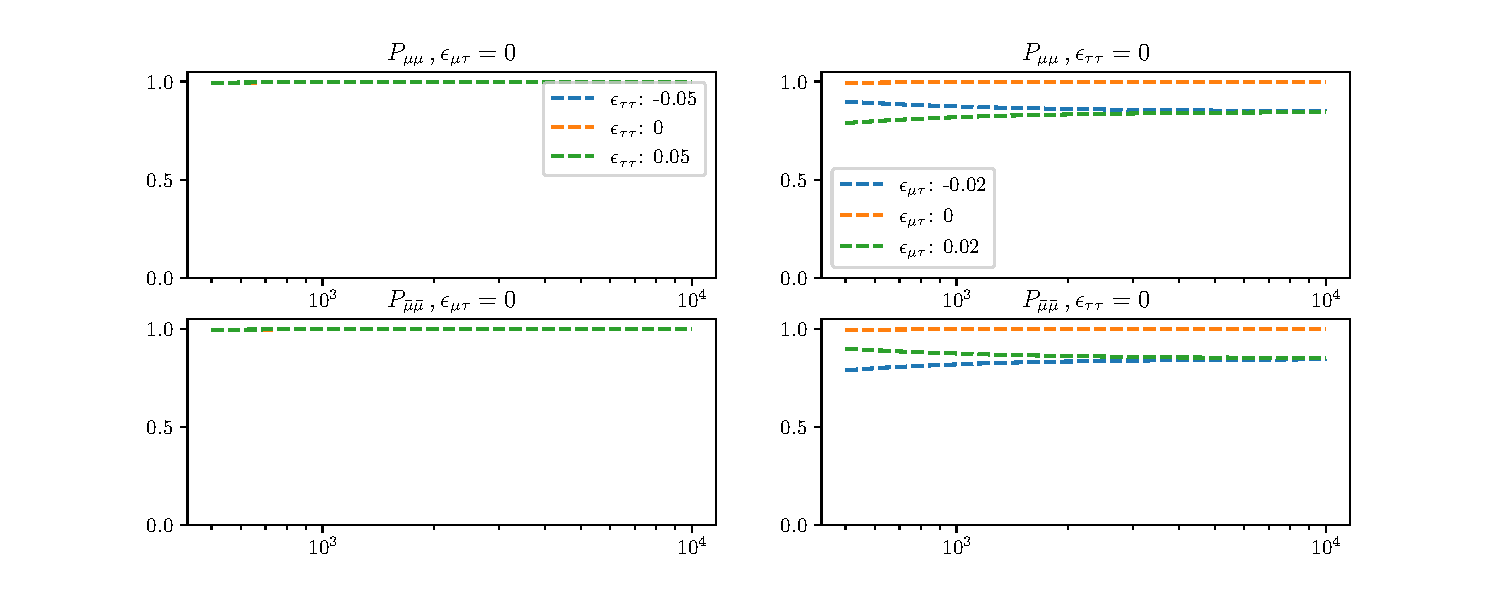
\includegraphics[width=1\textwidth, height=0.3\textheight]{figures/IC_NSI_probs.pdf}
    \caption{\emph{Top panels: }$\nm$ survival probability for different cases of the two NSI parameters $\ett$ and $\emt$
    \emph{Bottom panels: }$\anm$ survival probability for different cases of the two NSI parameters $\ett$ and $\emt$.
    In all plots, \ztrue = -1.}
    \end{center}
\end{figure}
\end{document}